\documentclass[a4paper]{article}

\usepackage{../mathstemplate}

\date{IV семестр, весна 2024 г.}
\title{Вариационное исчисление. Неофициальный конспект}
\author{Лектор: Роман Владимирович Романов \\ Конспектировал Леонид Данилевич \\ Редактировал Максим Лаунер}

\begin{document}
    \shorthandoff{"}
    \maketitle
    \tableofcontents
    \newpage
    \setcounter{lection}{0}
    \newlection{15 февраля 2023 г.}
    \section{Что мы будем изучать}
    Вариационное исчисление занимается поиском экстремумов в задаче, где число переменных бесконечно.

    Рассмотрим конечномерную ситуацию.
    Пусть имеется $f: M \map \R$, где $M$ --- какое-то многообразие.

    При поиске экстремумов формируются следующие направления:
    \numbers{
        \item Необходимое условие: $(\nabla f)(x) = 0$.
        \item Достаточное: форма $(D^2 f)(x)$ знакоопределён ($> < 0$).
        \item Поиск экстремумов сужения $f\big|_{N}$ на подмногообразие (метод множителей Лагранжа).
    }
    В случае вариационного исчисления вместо $M$ стоит некоторое бесконечномерное пространство, например, пространство функций.
    В основном мы будем заниматься аналогами 1 и 3 пунктов.

    Функция, которая в свою очередь задана на пространстве функций часто называется \emph{функционал}.
    Чтобы визуально различать <<обычные>> функции, и функционалы, образ точки $f$ под действием функционала $J$ будем обозначать $J[f]$.

    Пускай $X$ --- (пока произвольное) метрическое пространство, $J: X \map \R$ --- функция.
    \definition[$x \in X$ --- cтрогий локальный минимум]{
        $\exists \delta > 0: \forall y \in U_{\delta}(x): J[y] > J[x]$.
    }
    Аналогично определяются нестрогий минимум и максимумы.
    Также стоит вспомнить про существование глобальных строгих и нестрогих минимумов и максимумов.

    \example[Чего такого особенного в бесконечномерии?]{
        Пусть $X = \defset{f \in C[0, 1]}{f(0) = f(1) = 1}$, норма на $C[0, 1]$ определена формулой $\|f\| = \max\limits_{x \in [0, 1]}|f(x)|$.

        Пусть $J[f] \coloneqq \int\limits_{0}^{1}f^2(x)\d x$. Очевидно, $J$ непрерывен.

        Ясно, что $\forall f \in X: J[f] > 0$.
        С другой стороны, $\inf\limits_{f \in X}J[f] = 0$ --- можно рассматривать функции вида
        \[\begin{tikzpicture}
            \draw[->] (-1,0) -- (3,0) node[right] {$x$};
            \draw[->] (0,-1) -- (0,3) node[above] {$y$};
            \fill (2,0) circle (1.5pt) node[below] {$1$};
            \fill (0,2) circle (1.5pt) node[left] {$1$};
            \fill (0,0) circle (1.5pt) node[below left] {$0$};
            \draw[blue, line width=0.8pt] (0,2) -- (0.1,0);
            \draw[blue, line width=0.8pt] (0.1,0) -- (1.9,0);
            \draw[blue, line width=0.8pt] (1.9,0) -- (2,2);
            \draw[dashed] (0,2) -- (2,2);
            \draw[dashed] (2,0) -- (2,2);
        \end{tikzpicture}\]

        С третьей стороны, $X$ замкнуто: равномерный предел равномерных непрерывен, и условия на значения на концах уважают предел.
        Получается, в данном случае теорема Кантора не работает. В чём дело?

        Оказывается, проблема в том, что нет компактности: в бесконечномерном пространстве замкнутое ограниченное множество необязательно компактно.
    }
    \subsection{Интегральные функционалы}
    В дальнейшем мы будем рассматривать не произвольные функционалы, а ограничимся некоторым их подмножеством.

    Пусть задано непрерывное $L: [a, b] \times \R^n \times \R^n \map \R$, положим $J[u] \coloneqq \int\limits_{a}^{b}L(t, u(t), \dot{u}(t))\d t$.
    Мы будем заниматься множеством $X = C^1[a, b] = C^1([a, b] \map \R^n)$ (далее не будем указывать область значений, ясно из контекста) и его замкнутыми подмножествами.

    Такие $J$ называются \emph{интегральные функционалы}.
    Мы их изучаем, так как на них возможна богатая теория, и вместе с тем, интегральные функционалы часто встречаются в приложениях.
    \examples{
        \item $X = \defset{u \in C^1[a, b]}{u(a) = u_a, u(b) = u_b}, J[u] = \int\limits_{a}^{b}\sqrt{1 + (u')^2}\d x$ --- функционал длин графиков кривых, соединяющих две данные точки.
        \item $J = \int\limits_{a}^{b}(\frac{\dot u^2}{2} - V(u))\d x$, где $V$ --- заданная функция. В механике называется \emph{действием}.
    }
    Сначала убедимся, что они непрерывны.
    \note[О норме]{
        Для $f \in C^1[a, b]$: $\|f\| = \max\limits_{x \in [a, b]}|f(x)| + \max\limits_{x \in [a, b]}|f'(x)|$ --- очевидно норма. В дальнейшем мы всегда будем использовать такую норму для $C^1$.
    }
    \proposal{
        Пусть $X = C^1[a, b], L \in C([a, b] \times \R^n \times \R^n)$. Тогда интегральный функционал $J$ непрерывен на $X$.
        \provehere{
            Пусть $u, \tilde{u} \in X, \|u - \tilde{u}\| < \delta < 1$. \[\left|J[u] - J[\tilde{u}]\right| = \left|\int\limits_{a}^{b}L(x, \tilde{u}(x), \dot{\tilde{u}}(x)) - L(x, u(x), \dot{u}(x))\d x\right| \circlesign{\le}\]
            Заметим, что    $\|(x, \tilde{u}(x), \dot{\tilde{u}}(x)) - (x, u(x), \dot{u}(x))\|_{\R^{2n + 1}} < \delta$

            Рассмотрим $K = [a, b] \times \overline{B_{\|u\|_X + 1}} \times \overline{B_{\|u\|_{X} + 1}}$ --- компакт в $\R^{2n + 1}$.

            \[\circlesign{\le} \int\limits_{a}^{b}\omega_{L\big|_K}(\delta)\d x = (b - a)\omega_{L\big|_K}(\delta) \underset{\delta \to 0}\Map 0\]
            где $\omega$ --- модуль непрерывности. Он определён, так как $L\big|_K$ непрерывна на компакте.
        }
    }
    Пусть $X$ --- нормированное пространство (необязательно замкнутое), $J: X \map \R$.

    \definition[Производная функционала $J$ в точке $x$ по направлению $h \in X$]{
        \[\delta J[x, h] = \frac{\d}{\d t}\Big|_{t = 0}J[x + th]\]
        Иначе эту штуку называют \emph{вариация} $J$ по направлению $h$.
    }
    \properties[Вариация]{
    \item Однородность: $\delta J[x, ch] = c \cdot \delta J[x, h]$.
    \item Не следует ожидать аддитивность.
        Так, $\exists \delta J[x, h_1], \delta J[x, h_2]$ не влечёт существование $\delta J[x, h_1 + h_2]$, а если последнее и существует, то не обязано быть суммой.

        Примеры этого были в анализе, здесь бесконечномерной специфики нет.
        \item Как и в конечномерном анализе, в критической (экстремальной) точке вариация (коли существует) должна обращаться в нуль.

        А именно, $x \in X$ --- локальный экстремум $J$, тогда $\forall h: \exists \delta J[x, h] \then \delta J[x, h] = 0$.
        \provehere{
            Сужение $\alpha(t) = J[x + th]$ тоже имеет локальный экстремум, значит, если производная в $t = 0$ есть, то она равна нулю.
        }
    }

    \section{Формула первой вариации. Уравнение Эйлера --- Лагранжа}
    \subsection{Лемма Дюбуа-Реймона}
    \lemma[Дюбуа-Реймон]{\label{du-Bois-Reymond}
        Пускай $f \in C[a, b]$, и для всех $\omega \in C^1[a, b]$, таких, что $\omega(a) = \omega(b) = 0$, известно, что $\int\limits_{a}^{b}f \omega' = 0$.

        Тогда $f \equiv \const$.
        \provehere{
            Если бы $f$ сама была гладкой, то можно было бы интегрировать по частям. $\int f'\omega = 0 \then f' \equiv 0$ --- можно взять $\omega$, сосредоточенную там, где $f'$ одного знака.

            Мы надеемся, что $f$ --- константа, то есть равна своему среднему $\overline{f} \bydef \frac{1}{b - a}\int\limits_{a}^{b}f$.

            Определим $\omega$, интегрируя $f - \overline{f}$: $\omega(x) \coloneqq \int\limits_{a}^{x}\left(f(x') - \overline{f}\right)\d x'$. Понятно, что $\omega \in C^1$. Более того, несложно видеть, что $\omega(a) = \omega(b) = 0$.

            Подставим данную $\omega$ в посылку теоремы. \[0 = \int\limits_{a}^{b}f \omega' = \int\limits_{a}^{b}(f - \overline{f})\omega' = \int\limits_{a}^{b}(f - \overline{f})^2\d x\] Так как интеграл нуль, то получаем $f \equiv \overline{f}$.
        }
    }
    \subsection{Формула первой вариации}
    Опять $X = C^1[a, b]$, и функционал того же самого вида $J[u] = \int\limits_{a}^{b}L(t, u(t),\dot{u}(t))\d t$.
    \lemma[Формула первой вариации]{\label{vario-formula}
        Пусть $L \in C^1([a, b] \times \R^n \times \R^n)$.
        Градиент $L$ по второму и третьему аргументам будем обозначать $\nabla_u L$ и $\nabla_{\dot{u}} L$ соответственно, это векторы из $\R^n$.

        Тогда производная $J$ в точке $u$ по направлению $h$ существует, и равна \[\int\limits_a^b\left[\Big\langle(\nabla_u L)(t, u(t), \dot{u}(t)), h(t)\Big\rangle + \angles{(\nabla_{\dot{u}} L)(t, u(t), \dot{u}(t)), \dot{h}(t)}\right]\d t\]
        \provehere{
        $J[u + \tau h] - J[u] = \int\limits_{a}^{b}\left[ L\biggl(t, u(t) + \tau h(t) , \dot{u}(t) + \tau \dot{h}(t)\biggr) - L\biggl(t, u(t), \dot{u}(t)\biggr)\right]\d t$.

        Применяя формулу Лагранжа, получаем для некой $\tau_* = \tau_*(t) \in [0, \tau]$:
            \multline{J[u + \tau h] - J[u] = \tau\int\limits_{a}^{b} \biggl[\angles{ (\nabla_u L)(t, u(t) + \tau_* h(t), \dot{u}(t) + \tau_* \dot{h}(t)), h(t)} +\\+ \angles{(\nabla_{\dot{u}} L)(t, u(t) + \tau_* h(t), \dot{u}(t) + \tau_* \dot{h}(t)), \dot{h}(t)}\biggr]\d t}

            Поделив на $\tau$, получаем $\frac{J[u + \tau h] - J[u]}{\tau} = \int\limits_{a}^{b} \dots$ --- вот тот, что выше.

            Сперва разберёмся с первым слагаемым. Покажем, что \[\underbrace{\int\limits_{a}^{b}\angles{(\nabla_u L)(t, u(t) + \tau_* h(t), \dot{u}(t) + \tau_* \dot{h}(t)), h(t)}\d t}_{I} \underset{\tau \to 0}\Map \underbrace{\int\limits_{a}^{b}\angles{(\nabla_{u} L)(t, u(t), \dot{u}(t)), h(t)}\d t}_{\II}\]

            Модуль разности аргументов не превосходит $\tau_* \|h\|_{X}$.
            Отсюда $\|\nabla_u L(\dots) - \nabla_u L(\dots)\|_{\R^n} \le \omega_{L\big|_K}(\tau_* \| h\|_X)$, здесь $K \coloneqq [a, b] \times \overline{B_{\|u\| + \|h\|}} \times \overline{B_{\|u\| + \|h\|}}$ (мы считаем, что $\tau \le 1$, откуда $\tau_* \le 1$).

            Значит, $|(I) - (\II)| \le \int\limits_{a}^{b}\omega_{L\big|_K}(\tau_* \|h\|)\d t \le (b - a)\omega_{L\big|_K}(\tau \|h\|)\d t \underset{\tau \to 0}\Map 0$.

            Таким образом, у первого слагаемого под интегралом --- естественный предел.
            Аналогично со вторым слагаемым, получаем утверждение леммы.
        }
    }
    \subsection{Уравнение Эйлера --- Лагранжа}
    Пусть $u \in X$ --- экстремум.
    Тогда $\forall h \in X: \delta J[u, h] = 0$.

    Условие обнуления градиента --- некое уравнение на точку.
    Мы хотим уравнение на $u(t)$, избавимся от $h$.
    Подгоним под лемму Дюбуа-Реймона~(\cref{du-Bois-Reymond}).

    Введём $R(x) \coloneqq \int\limits_{a}^{x}(\nabla_u L)(t, u(t), \dot{u}(t))\d t$.
    Согласно~(\cref{vario-formula}) \[\delta J[x, h] = \int\limits_a^b \angles{\dot{R}(t), h(t)} + \angles{(\nabla_{\dot{u}} L)(t, u(t), \dot{u}(t)), \dot{h}(t)}\d t\]
    Поскольку $R(a) = 0$, интегрируя по частям, получим $\angles{R(b), h(b)} + \int\limits_{a}^{b}\Bigl\langle\underbrace{(\nabla_{\dot{u}}L)(t, u(t), \dot{u}(t)) - R(t)}_{\xi(t)}, \dot{h}(t)\Bigr\rangle\d t$

    И это равно нулю $\forall h \in C^1[a, b]$.
    Рассмотрим $h$, обращающийся на концах в ноль: $h(a)=h(b)=0$.
    Теперь $\int\limits_{a}^{b}\angles{\xi(t), \dot{h}(t)}\d t = 0$, и мы покомпонентно можем применить лемму Дюбуа-Реймона, получая $\xi(t) = C \equiv \const$.
    Но $R(t) \in C^1$, значит, $\nabla_{\dot{u}}L(t, u(t), \dot{u}(t)) \in C^1$ тоже.

    Дифференцируя $\xi$, получаем уравнение: $\frac{\d}{\d t}(\nabla_{\dot{u}} L)(t, u(t), \dot{u}(t)) - (\nabla_u L)(t, u(t), \dot{u}(t)) = 0$.
    Оно называется \emph{уравнение Эйлера --- Лагранжа}, это основное уравнение вариационного исчисления.

    \note{
        В случае общего положения уравнение Эйлера --- Лагранжа --- дифференциальное второго порядка, что соответствует $u \in C^2$: при вычислении $\frac{\d}{\d t}(\nabla_{\dot{u}} L)(t, u(t), \dot{u}(t))$ появится в общем случае вторая производная $u$.
        Такая ситуация, на самом деле, довольно общая: экстремаль <<регулярнее>>, чем произвольный элемент своего пространства.
    }
    \subsection{Случай свободных концов}
    Теперь рассмотрим совсем произвольную $h \in C^1$, получим уравнение ($C = \xi$ --- определена выше): \[0 = \delta J[u, h] = \angles{R(b), h(b)} + \int\limits_{a}^{b}\angles{C, \dot{h}(t)}\d t = \angles{R(b), h(b)} + \angles{C, h(b)} - \angles{C, h(a)}\]

    \numbers{
        \item Рассмотрим такую $h$, что $h(b) = 0, h(a) = C$.
        Для неё $\delta J[u, h] = -\|C\|^2$, значит, $\xi = C = 0$.

    Подставляя в определение $\xi$, получаем $R(a) = 0$, то есть $(\nabla_{\dot{u}} L)(a, u(a), \dot{u}(a)) = 0$.

    \item Теперь рассмотрим такую $h$, что $h(b) = R(b)$. В этом случае $\delta J[u, h] = \|R(b)\|^2 \then R(b) = 0$.
        Получили $(\nabla_{\dot{u}} L)(b, u(b), \dot{u}(b)) = 0$.
    }
    Итак, помимо уравнения Эйлера --- Лагранжа, мы получили два условия (но в разных точках) на уравнение второго порядка, можно надеяться, что хватит, чтобы найти решения (но это совсем не факт --- так, может существовать одно решение, а может их вовсе не быть, или быть бесконечно много).

    Подытожим в теорему.
    \theorem[Задача со свободными концами]{\label{free-ends}
        Пусть $L \in C^1([a, b] \times \R^n \times \R^n)$, пусть $X = C^1[a, b]$, пусть $u$ --- локальный экстремум $J$.

        Тогда
        \numbers{
            \item $\left(\nabla_{\dot{u}} L\right)(t, u(t), \dot{u}(t)) \in C^1[a, b]$.
            \item $\frac{\d }{\d t} \nabla_{\dot{u}} L = \nabla_{u} L$ --- уравнение Эйлера --- Лагранжа.
            \item $(\nabla_{\dot{u}} L)(a, u(a), \dot{u}(a)) = 0$
            \item $(\nabla_{\dot{u}} L)(b, u(b), \dot{u}(b)) = 0$
        }
    }
    \subsection{Случай фиксированных концов}
    Теперь обсудим, что происходит, если имеются граничные условия на функции из множества, по котором ищутся экстремумы функционалов.

    Рассмотрим $X = \defset{f \in C^1[a, b]}{f(a) = f_a, f(b) = f_b}$.
    Это не подпространство (не имеет линейной структуры), нельзя определить производную по направлению.

    Функционал $J: X \map \R$ задан той же формулой.

    Какая здесь характеризация локальных экстремумов?

    Рассмотрим $\tilde{J}: C^1[a, b] \map \R$ --- с той же формулой, что и $J$.
    Тогда $\forall u, h: \exists \delta\tilde{J}[u, h]$.

    С другой стороны, если $h \in C^1[a, b], h(a) = h(b) = 0$, то $\forall u \in X, t \in \R: u + th \in X$.
    Имеем право рассмотреть $J[u + th]$. Если $u$ --- локальный экстремум, то $\frac{\d }{\d t}\big|_{t = 0}J[u + th] = 0$.
    Она существует, так как это $\frac{\d}{\d t}\tilde{J}[u + th]$.

    Тем самым, такие функции $h$ прибавлять можно, будем это тоже называть вариацией: $\delta J[u, h]$ задаётся той же формулой.
    Дальше работает то же самое рассуждение, все действия те же самые, только при интегрировании по частям внеинтегральный член занулится, никаких дополнительных соотношений не возникнет.
    \theorem[Задача с фиксированными концами]{
        Пусть $L \in C^1([a, b] \times \R^n \times \R^n)$, пусть $X = \defset{f \in C^1[a, b]}{f(a) = f_a, f(b) = f_b}$, пусть $u$ --- локальный экстремум $J$. Тогда
        \numbers{
            \item $(\nabla_{\dot{u}} L)(t, u(t), \dot{u}(t)) \in C^1[a, b]$.
            \item $\frac{\d }{\d t} \nabla_{\dot{u}} L = \nabla_{u} L$ --- уравнение Эйлера --- Лагранжа.
        }
    }
    Заметим, что у нас по-прежнему два условия (теперь уже данные в самой задаче) и уравнение второго порядка, значит, по-прежнему, данных для решения задачи как раз столько, что стоит надеяться на получение решения.
    \newlection{29 февраля 2023 г.}
    Распишем чуть подробнее уравнение Эйлера --- Лагранжа, пусть для определённости функции скалярны ($d = 1$).
    Если все производные определены, то оно имеет вид
    \[\frac{\d}{\d t}\der{L}{\dot{u}} = \frac{\partial^2 L}{\partial t \partial \dot{u}} + \frac{\partial^2 L}{\partial u \partial \dot{u}}\dot{u} + \frac{\partial^2 L}{\partial \dot{u}^2}\ddot{u}\label{partial}\tag{$*$}\]
    Общая теорема~(\cref{free-ends}) говорит, что $\nabla_{\dot{u}}L$ имеет $C^1$ гладкость, однако совсем не утверждается, что при разложении~\eqref{partial} каждое слагаемое будет гладким, или даже просто будет существовать.
    И правда, такого и не наблюдается.
    \counterexample{
    Рассмотрим функционал $J[u] = \int\limits_{-1}^{1}u^2 (\dot{u} - 2x)^2 \d x$, где $X = \defset{u \in C^1[-1, 1]}{\arr{c}{u(-1) = 0\\u(1) = 1}}$
    и функцию $u \in X, u(t) = \all{0,& x\in [-1, 0] \\ x^2,& x \in [0, 1]}$. $u$ --- экстремаль, например, потому что это глобальный минимум.
    При этом $u \notin C^2$, хотя $\der{L}{\dot{u}} = 2u^2(\dot{u} - 2x) \equiv 0$ --- бесконечно гладкая.
    }
    Что нужно потребовать, чтобы все слагаемые~\eqref{partial} существовали?

    В примере сам лагранжиан $L(x, u, \dot{u}) = u^2(\dot{u} - 2x^2)$ --- бесконечно гладкий.
    Но $\ddot{u}$ можно выразить из~\eqref{partial} только если $\frac{\partial^2}{\partial \dot{u}^2}L \ne 0$.

    Следующее предложение формулируется в случае, когда $L$ задан на $[a, b] \times \R^d \times \R^d$; в общем случае сужения $L$ на некоторое подмножество принципиально ничего не поменяется.
    \proposal{
    Пусть $L \in C^2(\Omega)$, где $\Omega = [a, b] \times \R^d \times \R^d$, пусть $\det \left(\frac{\partial^2 L}{\partial \dot{u}^2}\right) \ne 0$ везде в $\Omega$.

    Пусть $u$ --- локальный экстремум функционала $J$. Утверждается, что $u \in C^2[a, b]$.
    \provehere{
        Введём функцию \begin{align*}\xi: [a, b] \times \R^d &\map \R^d\\ (t, v) &\mapsto (\nabla_{\dot{u}}L)(t, u(t), \dot{u}(t)) - (\nabla_{\dot{u}}L)(t, u(t), v)\end{align*}

    Согласно посылке теоремы, $\der{}{v} \xi \ne 0$ для всех $t, v$.
        Так как $u$ --- экстремум, то $\xi \in C^1$.

    По теореме о неявной функции $\forall t_0 \in (a, b): \exists \delta > 0: \defset{(t, v)}{\xi(t, v) = 0, |t - t_0| < \delta}$ --- график некоторой функции $v \in C^1\left((t_0 - \delta, t_0 + \delta) \map \R^d\right)$.
    Но $v \equiv \dot{u}\big|_{(t_0 - \delta, t_0 + \delta)}$. Значит, $u \in C^2(a, b)$.

    Случай концов ($t_0 = a, b$)--- упражнение.
    }
    }
    \section{Условные экстремумы}
    \emph{Согласно полуисторической, полулегендарный справке, некогда Дидона прибыла на берег некоего африканского государства, и потребовала, на основании своего высокого происхождения, выделить ей столько земли, сколько можно опоясать ремешком из шкуры одного быка\ldots}

    Напоминание конечномерного случая:
    пусть $\Omega \subset \R^d$ --- область, $f, g \in C^1(\Omega)$, $\mathcal{M} = \defset{x \in \Omega}{g(x) = 0}$.

    Заинтересуемся экстремумами сужения $f\big|_{\mathcal{M}}$.
    Пусть $x_0 \in \Omega$ -- экстремум.
    Построим кривую ${x:(-\eps,\eps)\map \Omega}$ так, что $x(0) = x_0$.
    Условие $g(x(t)) \equiv 0$ влечёт, что $f(x(t))$ имеет локальный экстремум в нуле.
    Другими словами, $\frac{\d}{\d t}\Big|_{t = 0}f(x(t)) = \angles{(\nabla f)(x_0), \dot{x}(t)} = 0$.

    Поскольку кривую можно выбрать с любым вектором скорости, то $(\nabla f)(x_0) \perp T_{x_0}\mathcal{M}$.
    Если $(\nabla g)(x_0) \ne 0$ в $x_0$, то $T_{x_0}\mathcal{M}$ --- пространство коразмерности $1$.
    Найдём какой-нибудь вектор, перпендикулярный $\mathcal{M}$.
    Это как раз градиент: $g(x(t)) = 0 \then \angles{(\nabla g)(x_0), \dot{x}} = 0$.

    Иными словами $\exists \lambda\in\R: \nabla(f - \lambda g)(x_0) = 0$.
    Далее для поиска экстремумов ищут критические точки $f - \lambda g$, выделяют те, которые в $\mathcal{M}$, а с обнулениями градиента $g$ разбираются отдельно.
\ok
    Пускай $X$ --- нормированное замкнутое пространство, $G \in C^1(X)$ --- задающий условие функционал.
    Расшифруем условие $G \in C^1(X)$:
    \bullets{
    \item $\forall x \in X: \exists G'(x) \in X^*: |G(x + s) - G(x) - G'(x)s| = o(\|s\|)$ --- \emph{сильная дифференцируемость} в точке $x$.
    \item Определённое в предыдущем пункте отображение $G': X \map X^*$ непрерывно.
    }
    Для применения метода множителей Лагранжа нам понадобится лемма, утверждающая, что в направлении всякого вектора из $\Ker G'(x_0)$ можно пустить путь --- как в конечномерном случае.
    \lemma{\label{path-with-given-vector}
    Пусть $x_0 \in \mathcal{M} \coloneqq \defset{x \in X}{G(x) = 0}$.
    Пусть $G'(x_0) \ne 0$.

    Тогда $\forall h \in \Ker G'(x_0): \exists x \in C^1((-\delta,\delta) \map \mathcal{M}): x(0) = x_0, \dot{x}(0) = h$.
    \provehere{
        Зафиксируем произвольный $\xi \notin \Ker G'(x_0)$. Определим $r(t, \tau) \coloneqq G[x_0 + t\xi + \tau h]$. Ясно, что $r \in C^1\left(\left[-\eps, \eps\right] \times [-\eps, \eps]\right)$.

        $r(0, 0) = 0$, $\der{r}{t}(0, 0) = G'[x_0]\xi \ne 0$.
        Применяя теорему о неявной функции, получаем $\exists \delta > 0: \defset{(t, \tau)}{\tau \in (-\delta, \delta), r(t, \tau) = 0}$ --- график $C^1$ функции $t = t(\tau)$, где $t: (-\delta, \delta) \map \R$.

        Проверим, что $x: \tau \mapsto x_0 + t(\tau)\xi + \tau h$ --- искомая кривая:
    \numbers{
    \item По построению $x: (-\delta, \delta) \map \mathcal{M}$ --- класса $C^1$.
    \item Дифференцируя тождество $G[x(t)] = 0$ в точке $t = 0$, получаем $G'[x(0)] \cdot \dot{x}(0) = 0$, значит, $\dot{x}(0) \in \Ker G'[x_0]$.
        С другой стороны, $\dot{x}(0) = \dot{t}(0)\xi + h$, откуда $\dot{t}(0) = 0$ (ведь $\xi \notin \Ker G'[x_0]$).
        Тем самым, $\dot{x}(0) = h$.\qedhere
    }
    }
    }
    Пускай $F \in C^1(X), x_0 \in \mathcal{M}$ --- точка локального экстремума сужения $F\big|_{\mathcal{M}}$.

    Рассмотрим только что построенную кривую $x(\tau)$ ($x'(0) = h$).
    Так как $x_0$ --- экстремаль, то в частности должно быть $\frac{\d}{\d \tau}\Big|_{\tau = 0}F[x(\tau)] = 0$.
    С другой стороны, это равно $F'[x_0]\cdot h$.

    Значит, $\Ker G'[x_0] \subset \Ker F'[x_0]$, причём $\exists \lambda \in \R: (F'[x_0] - \lambda G'[x_0]) = 0$ --- и $F'$, и $G'$ обнуляются на пространстве коразмерности $1$.
    Формальнее, выберем $\eta \notin \Ker G'[x_0]$, и разложим \[\forall h \in X: h = \underbrace{\left(h - \frac{G'[x_0]h}{G'[x_0]\eta}\eta\right)}_{\in \Ker G'[x_0]} + \frac{G'[x_0]h}{G'[x_0]\eta}\eta\]
    Значит, $(F'[x_0] - \lambda G'[x_0])(h) = \frac{G'[x_0]h}{G'[x_0]\eta}\cdot (F'[x_0] \eta - \lambda G'[x_0]\eta)$.
    Видно, что подойдёт $\lambda = \frac{F'[x_0]\eta}{G'[x_0]\eta}$.

    Получилась теорема:
    \theorem{\label{lagrangian-multipliers}
    Пускай $F, G \in C^1(X)$, пускай $x_0$ --- точка локального экстремума $F$ на $\mathcal{M} \coloneqq \defset{x \in X}{G[x] = 0}$, пусть $G'[x_0] \ne 0$.

    Тогда $\exists \lambda \in \R: \forall h \in X: \delta(F - \lambda G)[x_0, h] = 0$ (отметим, что так как $F, G \in C^1$, то $\exists \delta (F - \lambda G)$.)
    }
    \exercise{Задача с фиксированными концами}
    \subsection{Случай нескольких условий}
    Даны $F, G_1, \dots, G_n \in C^1(X), \mathcal{M} \coloneqq \defset{x \in X}{G_1[x] = \dots = G_n[x] = 0}$.

    Образуем линейный оператор $\mathbb{G}'[x_0] = \vect{G'_1[x_0] \\ \vdots \\ G'_n[x_0]}: X \map \R^n$ по правилу $\mathbb{G}'[x_0]h = \vect{G'_1[x_0]h \\ \vdots \\ G'_n[x_0]h}$.

    \theorem{\label{different-boundaries}
    Пусть $x_0$ --- точка локального экстремума $F$ на $\mathcal{M}$, пусть $\Ran \mathbb{G}'[x_0] = \R^n$ (иными словами $\sum\limits_{j=1}^{n} c_j G'_j[x_0] = 0 \then \forall j: c_j = 0$) ($\Ran$ (от англ. range) --- образ).

    Тогда $\exists \lambda_1, \dots, \lambda_n \in \R: \forall h \in X: \delta(F - \sum \lambda_j G_j)[x_0, h] = 0$
    \provehere{
    \indentlemma{
        В тех же предположениях невырожденности $\Ran \mathbb{G}'(x) = \R^n$.
        Пусть $h \in \bigcap\limits_{j = 1}^{n}\Ker G_j'[x_0]$.
        Тогда $\exists x: (-\delta, \delta) \map \mathcal{M}, x \in C^1, x(0) = x_0, \dot{x}(0) = h$.
    }{
        Аналогично~(\cref{path-with-given-vector}), тоже теорема о неявной функции.
    }
    Полностью аналогично скалярному случаю $n = 1$.
    }
    }
    \note{
    Можно попробовать применить скалярную теорему с $n = 1$ к функционалу $G[x] = \sum\limits_{i=1}^{n} G_i^2[x]$.
        Однако это ничего не даст, так как $G'[x] = 0$ везде на $\mathcal{M}$.
    }
    \exercise{Доказать аналогичное утверждение для задачи с фиксированными концами.}
    Теперь применим~(\cref{different-boundaries}) к случаю интегральных функционалов.
    \theorem{
    Пускай $L, r_1, \dots, r_n \in C^1([a, b]\times\R^d \times \R^d)$, и определены $J[u] \coloneqq \int\limits_{a}^{b}L(t, u(t), \dot{u}(t))\d t$, $R_j[u] \coloneqq \int\limits_{a}^{b}r_j(t, u(t), \dot{u}(t))\d t$.

    Пусть $u_0$ --- точка локального экстремума $J\big|_{\bigcap \Ker R_j}$; оператор $\R(u_0) \coloneqq \vect{R_1'(u_0) \\ \vdots \\ R_n'(u_0)}$ имеет полный ранг (можно явно выразить производные при помощи~(\cref{vario-formula}))).
        \comment{Вообще, если я правильно понимаю, лемма даёт производные по Гато, что не гарантирует существование производных по Фреше.
        Тем не менее, несложно видеть, что доказательство не меняется, если считать производные по Фреше --- все оценки прячутся в $o(\|h\|)$.
        }

    Тогда
    \numbers{
        \item $\exists \lambda_1, \dots, \lambda_n: \nabla_{\dot{u}}(L - \sum \lambda_j r_j)(t, u_0(t), \dot{u}_0(t)) \in C^1[a, b]$.
        \item Выполнено уравнение Эйлера --- Лагранжа: $\frac{\d}{\d t}\nabla_{\dot{u}}(L - \sum \lambda_j R_j) = \nabla_u (L - \sum \lambda_j R_j)$
        \item $\nabla_{\dot{u}}(L - \sum \lambda_j r_j)\Big|_{t = a} = \nabla_{\dot{u}}(L - \sum \lambda_j r_j)\Big|_{t = b} = 0$.
    }
    \provehere{
        Вытекает из доказательства~(\cref{free-ends}) (там использовалось только то, что вариация обращается в нуль, а не то, что $u_0$ --- экстремаль) и~(\cref{lagrangian-multipliers}).
    }}
    \example{
    Пускай $\Omega \subset \R^3$ --- ограниченная область, граница которой --- поверхность класса $C^1$.
        Введём пространство непрерывных на этой границе функций $X \coloneqq C(\partial \Omega)$.

    Заведём $J[\sigma] \coloneqq \iint\limits_{\partial \Omega \:\partial\Omega}\frac{\sigma(x)\sigma(y)\d S(x)\d S(y)}{|x - y|}$.

    $J$ непрерывен на $X$, поскольку $\xi: y \mapsto \int\limits_{\partial \Omega}\frac{\sigma(x)}{|x - y|}\d S(x)$ непрерывно.
    \[J[\sigma + s] - J[\sigma] = 2\iint\limits_{\partial \Omega \:\partial\Omega}\frac{s(x)\sigma(y)}{|x - y|}\d S(x)\d S(y) + \bigO(\|s\|^2_C)\]

    Также $s \mapsto \int\limits_{\partial\Omega}s(x)\xi(x)\d x$ непрерывен, откуда $J$ --- даже функционал класса $C^1(X)$.
    }
    \newlection{14 марта 2023 г.}
    Заинтересуемся экстремумами с постоянным значением $G[\sigma] = \int\limits_{\partial \Omega}\sigma(x)\d x$.
    Решение будет отвечать распределению зарядов на поверхности, минимизирующее энергию системы --- физический принцип говорит, что конечное положение экстремально.

    Уже проверили, что $J, G \in C^1(X)$.

    Пусть $\sigma$ --- экстремаль $J\big|_{\{\sigma \in X|G(\sigma) = Q\}}$.
    Тогда $\forall h \in X$: $\delta (J - \lambda G)[\sigma, h] = 0$.
    Посчитаем \multline{\delta (J - \lambda G)[\sigma, h] = (J - \lambda G)[\sigma + h] - (J - \lambda G)[\sigma] =\\= 2\int\limits_{\partial \Omega}\int\limits_{\partial \Omega}\frac{\sigma(x)h(y)}{|x - y|}\d S(x)\d S(y) - \lambda \int\limits_{\partial \Omega} h(y)\d S(y) + \int\limits_{\partial \Omega}\int\limits_{\partial \Omega}\frac{h(x)h(y)}{|x - y|}\d S(x)\d S(y)}
    Третье слагаемое $\bigO(\|h\|^2_X)$: $\iint\frac{1}{|x - y|}$ сходится.
    Заметим, что остальная часть --- линейный функционал от $h$, где коэффициент непрерывен от $\sigma$.
    Это в точности значит, что $J \in C^1$.
    \[J[\sigma + h] -J[\sigma] = l_\sigma(h) + o(\|h\|)\text{, где }l_\sigma: h \mapsto \iint\limits_{\partial \Omega\times\partial \Omega} \frac{\sigma(x)h(y)}{|x - y|}\d S(y) = \int\limits_{\partial \Omega} \xi(y)h(y)\d S(y)\]
    Запишем условие экстремальности:
    \[\forall h: \delta(J - \lambda G)[\sigma, h] = 2\int h(y)\d S(y)\left(2\int \frac{\sigma(x)\d S(x)}{|x - y|} - \lambda\right) = 0\]
    По <<нулевой лемме Дюбуа-Реймона>>, выражение в скобочках должен быть всегда нулём.

    Получили
    \encircle{\lambda = 2\int \frac{\sigma(x)\d S(x)}{|x - y|}}
Экстремаль $\sigma$ ищется, как решение <<интегрального уравнения>>: заведём $K: f \mapsto \int \frac{f(x)\d S(x)}{|x - y|}$, это ограниченный непрерывный интегральный оператор.
    Таким образом, $\sigma$ --- решение $K \sigma = \frac{\lambda}{2}\1$.

    Иными словами, потенциал, создаваемый распределением заряда на самой поверхности постоянен.
    Такая постановка задачи не очень естественна --- например, бывают точечные заряды.
    Естественнее было бы рассматривать задачи вида $\sigma$ --- борелевская мера на $\partial \Omega$, $J[\sigma] = \int\frac{\d\sigma(x)\d \sigma(y)}{|x - y|}$.
        Тут уже уместно задавать вопросы о существовании интеграла, сходимости, и прочем, мы не будем это выяснять по причине нехватки аппарата.
% Вот если бы вы выбрали курс по потенциалам, \textbf{А вы не выбрали!}, то там бы вам рассказали об этом подробнее
    \section{Функционалы на кривых}
    В задаче Дидоны ответом является некоторая кривая, а кривая, в зависимости от того, как выбрать параметр, может не реализовываться, как график функции.
    С другой стороны, хотим независимость от параметризации, потому что зачем.
    \definition[Кривая $\gamma \in C$]{Непрерывное отображение $\gamma: [a, b] \map \R^n$.}
    \definition[Параметризованная кривая $\gamma$]{$\forall x \in [a, b]: \gamma'(x) \ne 0$.}
    \definition[Кривая $\gamma$ класса $C^j$]{Кривая $\gamma \in C^j$.}
    Пусть $\gamma_1: [a_1, b_1] \map \R^n, \gamma_2: [a_2, b_2] \map \R^n$ --- две параметризованные кривые.
    \definition[Эквивалентность кривых $\gamma_1$ и $\gamma_2$]{ Диффеоморфизм $\kappa \in C^j([a_1, b_1] \map [a_2, b_2])$, такой, что $\gamma_1 = \gamma_2 \circ \kappa$ и $\forall x: \kappa'(x) > 0$.
    Класс эквивалентности относительно данного отношения зовётся \emph{ориентированная кривая}. }

    За $\Gamma^j$ обозначим множество ориентированных кривых, представители которых --- кривые класса $C^j$.
    Ещё используют $\Gamma^j[a, b]$.

    Пускай $\Fc \in C(\R^n \times \R^n)$, пусть она однородная порядка $1$ по второму аргументу: \[\forall \lambda > 0: \Fc(z, \lambda w) = \lambda \Fc(z, w)\]
    Пусть $\gamma: [a_\gamma, b_\gamma] \map \R^d$ --- кривая класса $C^1$.
    Определим $J[\gamma] \coloneqq \int\limits_{a_\gamma}^{b_\gamma}\Fc[\gamma(t), \dot{\gamma(t)}]\d t$.

    \proposal{
        В этой ситуации $J$ задаёт функционал на $\Gamma^1$.
    \provehere{
        Пусть $\gamma_1: [a_1, b_1] \map \R^d, \gamma_2: [a_2, b_2] \map \R^d$ --- два эквивалентных представителя.
        
    \multline{J[\gamma_1] = \int\limits_{a_1}^{b_1} \Fc[\gamma_1(t), \dot{\gamma}_1(t)]\d t = \int\limits_{a_1}^{b_1} \Fc [\gamma_2(\kappa(t)), \dot{\kappa}(t) \cdot \dot{\gamma}_2(\kappa(t))]\d t = \\
    =\int\limits_{a_1}^{b_1} \Fc [\gamma_2(\kappa(t)), \dot{\gamma}_2(\kappa(t))]\dot{\kappa}(t)\d t = \left\|\arr{c}{\tau = \kappa(t) \\ \d \tau = \dot{\kappa}(t)\d t}\right\| = \int\limits_{a_2}^{b_2} \Fc[\gamma_2(\tau), \dot{\gamma}_2(\tau)]\d \tau\qedhere}
    }
    }
    \examples{
    \item $\Fc(z, w) = |w|$.
        Функционал $J$ --- длина кривой
    \item $\Fc(z, w) = |w|\cdot f(z)$, где, например, $d = 2$ (кривая плоская), $f(z) = z_2^{\alpha}$ (здесь $z = \vect{z_1\\z_2}$).
    \bullets{
        \item При $\alpha = 0$ это предыдущий случай.
        \item При $\alpha = -1$ это длина в гиперболической плоскости (в модули Пуанкаре в верхней полуплоскости).
        \item При $\alpha = 1$ это координата центра масс кривой, а ещё --- площадь поверхности вращения.
    \item При $\alpha = -\frac{1}{2}$ это время, требуемое шарику, чтобы скатиться по жёлобу данной формы.
    }
    }
    Пусть $L \in C([a, b] \times \R^n \times \R^n)$, $X = C^1[a, b]$, $J[u] = \int\limits_{a}^{b}L(t, u(t), \dot{u}(t))\d t$.
    Превратим последний в функционал на кривой.
    Заведём $\Fc: \R^{n+1}\times\R^{n+1}, \Fc(z, w) = L(z_1, z_2, \dots, z_{n+1}, \frac{w_2}{|w_1|}, \dots, \frac{w_{n+1}}{|w_1|})|w_1|$.
    Он имеет требуемую однородность.
    Типа сопоставим функции $u(t)$ кривую $\gamma_u: t \mapsto (t, u(t))$.
    % Потолок пробили, но сверху постучали

    Рассмотрим $\tilde{J}[\gamma] \coloneqq \int\Fc(\gamma(t), \dot{\gamma}(t))\d t$, утверждается, что если $L$ <<разумная>>, то $\tilde{J}$ --- функционал на кривых.
    \proposal{
    $\tilde{J}[\gamma_u] = J[u]$.\provehere{$\dot{\gamma}_u(t) = (1, \dot{u}(t))$.}
    }
%    Сформулируем некоторое техническое утверждение, которым будем пользоваться в меньшей общности, и докажем не здесь, но сформулируем сейчас
    \statement{
    Пусть $\Fc \in C^2(\R^n \times (\R^n \sm \{0\})) \cap C(\R^n \times \R^n)$.

    Пусть $\forall \lambda > 0: \Fc(z, \lambda w) = \lambda\Fc(z, w)$.

        Пусть $\gamma \in \Gamma^2$, $\gamma: [a_\gamma, b_\gamma]\map \R^d$.
        $J[\gamma] = \int\limits_{a_\gamma}^{b_\gamma} \Fc[\gamma, \dot{\gamma}]\d t$, $E\{\gamma\} \coloneqq (\nabla_{z} \Fc)(\gamma, \dot{\gamma}) - \frac{\d}{\d t}(\nabla_w \Fc)(\gamma, \dot{\gamma})$.
        Определение осмысленно, так как кривая параметризована, и $\dot{\gamma} \ne 0$, а $\Fc \in C^2(\dots)$.
        % Пределы не стоят намеренно, так как параметризации могут разниться

        Теперь пусть $s \in C^2\left([a, b] \times [-\eps, \eps] \map \R^n\right)$, и пусть $s(\_, \tau)$ --- параметризованная кривая.
        Тогда $\frac{\d}{\d \tau}J[s(\_, \tau)] = \int\limits_{a}^{b}E\{s(x, \tau)\}\d x + \angles{(\nabla_{w}\Fc )(s(x, \tau), \der{s}{x}(x, \tau)), \der{s}{\tau}}\Big|_{x = a}^{x = b}$
    \provehere{
        Упражнение.
    }
    }
    \lemma{
        Пусть $\gamma_1 \sim \gamma_2$ --- представители кривой $\gamma \in \Gamma^2$ ($\gamma_1 = \gamma_2 \circ \kappa$).
        Тогда $(E\{\gamma_1\})(x) = \kappa'(x)\left(E\{\gamma_2\}\right)(\kappa(x))$.
        \provehere{
            \multline{
                E\{\gamma_1\}(x) = (\nabla_z \Fc) (\gamma_1(x), \gamma'_1(x)) - \frac{\d}{\d x}(\nabla_w \Fc)(\gamma_1(x), \dot{\gamma}_1(x)) =\\= \kappa'(x)(\nabla_z \Fc)\left(\gamma_2(\kappa(x)), \gamma_2'(\kappa(x))\right) - \frac{\d}{\d x}(\nabla_w \Fc)(\gamma_1(x), \dot{\gamma}_1(x))\circlesign{=}}
            Дифференцируя по $w$ равенство $\Fc(z, \lambda w) = \lambda \Fc(z, w)$, получаем $\lambda(\nabla_w \Fc)(z, \lambda w) = \lambda (\nabla_w\Fc)(z, w)$
            \[\circlesign{=}\kappa'(x)(\nabla_z \Fc)\left(\gamma_2(\kappa(x)), \gamma_2'(\kappa(x))\right)-\kappa'(x)\frac{\d}{\d s}\Big|_{s = \kappa(x)}(\nabla_w\Fc)(\gamma_2(s), \gamma_2'(s)) = \kappa'(x)\cdot (E\{\gamma_2\})(\kappa(x))\]
        }
    }
    \corollary{
    $E\{\gamma_1\} \equiv 0 \iff E\{\gamma_2\} \equiv 0$ при $\gamma_1 \sim \gamma_2$.
    }
    Заведём метрику на $\Gamma^2$, чтобы определить экстремумы.
    Пусть $\xi: [a_\xi, b_\xi] \map \R^d$ и $\nu: [a_\nu, b_\nu] \map \R^d$ --- представители $\gamma_\xi, \gamma_\nu \in \Gamma^2$.

    Перепараметризуем $\xi$ и $\nu$ так, что они определены на $[0, 1]$, и их скорости постоянны: $|\dot{\xi}| \equiv \const, |\dot{\nu}| \equiv \const$.

    Положим $\|\gamma_\xi - \gamma_\nu\| = \|\xi - \nu\|_{C^2[0, 1]}$.
    \exercise{
    Проверить, что это метрика на $\Gamma^2$.
    }
    С метрикой также пришли всевозможные локальные, глобальные, строгие, нестрогие, минимумы и максимумы.
    \theorem{
    Пусть $\gamma \in \Gamma^2$ --- локальный максимум $J$, непрерывная $\Fc \in C^2(\R^n \times (\R^n \sm \{0\}))$, $\forall \lambda > 0: \Fc(z, \lambda w) = \lambda \Fc(z, w)$.

    Пусть $\gamma_a, \gamma_b \in \R^n, \mathcal{D} = \defset{\gamma \in \Gamma^2}{\gamma(a_\gamma) = \gamma_a, \gamma(b_\gamma) = \gamma_b}$ ($J$ задаётся на пространстве $\mathcal{D}$).
    
    Тогда $E\{\gamma\} = 0$.
    \provehere{
    Рассмотрим $\gamma + \tau h$, где $h(a_\gamma) = h(b_\gamma) = 0$, $h: [a_\gamma, b_\gamma] \map \R^d, h \in C^2$

        Так как $\dot{\gamma}(s) \ne 0$, то $\|\dot{\gamma}(s)\| \ne 0$, и при достаточно малых $\tau: \min\|\dot{\gamma} + \tau \dot{h}\| > \eps$.
        Значит, при подстановке мы попадём в область, где $\Fc \in C^2$, и существует $\frac{\d}{\d \tau}\big|_{\tau = 0}J[\gamma + \tau h] = 0$,

    Раз $\gamma$ --- экстремум, то производная равна нулю.
    \[J[\gamma + \tau h] - J[\gamma] = \tau\int\limits_{a_\gamma}^{b_\gamma}\left[\angles{(\nabla_z\Fc)(\gamma, \dot{\gamma}), h} + \angles{(\nabla_w\Fc)(\gamma, \dot{\gamma}), h'}\right]\d t + \bigO(\tau^2)\]
    Интегрируя по частям, получаем $\int\limits_{a}^{b}\angles{E\{\gamma\}, h}\d t + 0 + \bigO(\tau^2)$.
        Применяя <<нулевую лемму Дюбуа-Реймона>>, получаем $E\{\gamma\} = 0$.
    }
    }
    Таким образом, мы доказали, что чтобы показать экстремальность кривой $\gamma$, достаточно проверять экстремальность любой её перепараметризации, а экстремальность проверяется при помощи уравнения, аналогичного уравнению Эйлера --- Лагранжа: $E\{\gamma\} = 0$.
    \newlection{28 марта 2024 г.}
    \section{Условия трансверсальности. Задача Лагранжа}
    Пусть $J$ --- функционал на кривых, концы которых должны находиться на двух заданных многообразиях $M_1, M_2 \subset \R^n$.
    Считаем, что $J, M_1, M_2 \in C^1$.
    Функционал рассматривается на пространстве $X = \defset{\gamma \in \Gamma^2}{\gamma(a_\gamma) \in M_1, \gamma(b_\gamma)\in M_2}$ и задан обычной интегральной формулой
    \[J[\gamma] = \int\mathcal{F}[\gamma, \dot{\gamma}]\d t\text{, где }\mathcal{F} \in C^2(\R^n \times (\R^n \sm \{0\})) \cap C(\R^n \times \R^n), \forall \lambda > 0: \Fc(z, \lambda w) = \lambda \Fc(z, w)\]

    Пусть $\gamma_0$ --- локальный экстремум $J$ на $X$.
    Тогда $\gamma_0$ --- экстремум на $\defset{\gamma \in X}{\gamma(a_\gamma) = \gamma_0(a_{\gamma_0}), \gamma(b_\gamma) = \gamma_0(b_{\gamma_0})}$, следовательно, $E\{\gamma_0\} = 0$.

    Изучим граничные условия.
    Теперь кривая вида $\gamma_0 + \tau h$ не лежит в $X$, поэтому просто изучить вариацию не получится.

    Попробуем подвигать один из концов кривой так, чтобы он оставался на многообразии, и через некоторое расстояние подвинутая кривая сливалась с изначальной.

    Запишем это формулами.
    Пусть $a \coloneqq a_{\gamma_0}, b \coloneqq b_{\gamma_0}$, пусть $r: (-\eps, \eps) \map M_1, r \in C^2, r(0) = \gamma_0(a)$.
    Пусть $\delta > 0$ мало, $c \in (0, b - a]$.
    Рассмотрим $s$ вида $s(t, \tau) = \all{\gamma_0(t) + (r(\tau) - \gamma_0(a)), & t \in [a, a + \delta) \\ \gamma_0(t),& t \in [b - c, b]}$.
    Потребуем $s(\_, 0) = \gamma_0$ и $s \in C^2([a, b] \times (-\eps, \eps))$, $s(t, \_) \in X$.
    Также потребуем, чтобы $\forall t, \tau: \der{s}{t} \ne 0$, то есть кривая $s(\_, \tau)$ должна быть регулярной.

    \example{
    Пусть $h$ --- шапочка, как ниже, тогда подойдёт $s(t, \tau) = \gamma_0(t) + h(t) \cdot (r(\tau) - r(0))$.
        \[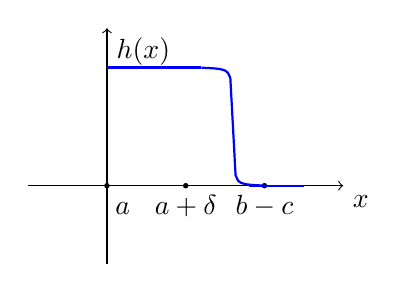
\begin{tikzpicture}
             \draw[->](-1, 0) -- (3, 0) node[below right] { $x$ };
             \draw[->](0, -1) -- (0, 2) node[below right] { $h(x)$ };
             \fill (0, 0) circle (1pt);
             \node at (0.2, -0.09) [below] {$a$};
             \fill (1, 0) circle (1pt) node[below] {$a + \delta$};
             \fill (2, 0) circle (1pt) node[below] {$b - c$};
             \draw[blue, thick] (0, 1.5) -- (1.2, 1.5);
             \draw[scale=1,domain=-0.4:0.4,blue,thick] plot ({1.6+\x},{0.75 - atan(\x * 100) / 90 * 0.76});
             \draw[blue, thick] (1.8, 0) -- (2.5, 0);
        \end{tikzpicture}\]
    }
    Так как $\gamma_0$ --- экстремум, то $J[s(\_, \tau)]$, как функция от $\tau$, имеет экстремум при $\tau = 0$.
    Положим $f(\tau) = J[s(\_, \tau)]$, и посчитаем $f'(\tau)$, приблизив разность первым членом ряда Тейлора:
    \[f(\tau) - f(0) = \int\angles{\nabla_u \mathcal{F}, s - \gamma_0} + \angles{\nabla_{\dot{u}}\mathcal{F}, \dot{s} - \dot{\gamma}_0} + \bigO(\|s(\_, \tau) - \gamma_0\|^2_{\Gamma^2}) \circlesign{=}\]
    Формула применима, так как $\Fc \in C^2(\R^n \times (\R^n \sm \{0\}))$, и $\dot{u}$ отделён от нуля.

    $\der{s}{t} \neq 0$, равномерно отделена от нуля, а отрезок фиксирован, откуда $\bigO\left(\|s(\_, \tau) - \gamma_0\|_{\Gamma^2}\right) \equiv \bigO\left(\|s(\_, \tau) - \gamma_0\|_{C^2}\right)$.

    Теперь применим формулу Тейлора по $\tau$:
    \multline{\circlesign{=}\tau\int\limits_{a}^{b}\left[\angles{\nabla_u\mathcal{F}, \der{s}{\tau}(\_, 0)} + \angles{\nabla_{\dot{u}}\mathcal{F}, \der{\dot s}{\tau}(\_, 0)}\right]\d \tau + \bigO(\tau^2) =\quad\text{(интегрируем по частям)}\\
        = \tau\left[\int\limits_{a}^{b}\angles{E\{\gamma_0\}, \der{s}{\tau}(\_, 0)}\d \tau - \angles{\nabla_{\dot u} \Fc, \der{s}{\tau}(a, 0)}\right]  + \bigO(\tau^2) =\\
        =- \tau\angles{\nabla_{\dot{u}}\mathcal{F}(\gamma_0)(a), \der{s}{\tau}(a, 0)} + \bigO(\tau^2)}
    Так как по построению $\der{s}{\tau}(b, 0) = 0$, то внеинтегральный член в $b$ равен нулю.
    При этом $\der{s}{\tau}(a, 0) = \der{r}{\tau}(0)$.
    Итак,
    \[f'(0) = 0 \then \angles{(\nabla_{\dot{u}}\mathcal{F})(\gamma_0)(a), \der{r}{\tau}(0)} = 0\]
    Так как $r$ --- любая кривая через $\gamma_0(a)$, то $(\nabla_{\dot{u}}\mathcal{F})(\gamma_0)(a) \perp T_{\gamma_0(a)}M$.

    Аналогично со вторым концом.

    Запишем всё это в теорему:
    \theorem{
    Пускай $J$ --- функционал на кривой ($\mathcal{F} \in C(\R^n \times \R^n) \cap C^2(\R^n \times (\R^n \sm \{0\}))$), как водится, $\forall \lambda > 0: \Fc(z, \lambda w) = \lambda \Fc(z, w)$, $M_1, M_2 \subset \R^n$ --- многообразия класса $C^1$, пусть $\gamma_0$ --- локальный экстремум $J$ на $X$.

    Тогда
    \numbers{
    \item $E\{\gamma_0\} = 0$.
    \item $\all{(\nabla_{\dot{u}}\mathcal{F})(\gamma_0)(a) \perp T_{\gamma_0(a)}M_1 \\ (\nabla_{\dot{u}}\mathcal{F})(\gamma_0)(b) \perp T_{\gamma_0(b)}M_2}$ --- условия трансверсальности.
    }
    }
    \examples{
    \item $\mathcal{F}(z, w) = |w|$.
    Минимум этого функционала --- расстояние от $M_1$ до $M_2$.

        Условия из теоремы означают, что $\dot{\gamma}_0(a) \perp T_{\gamma(a)}M_1, \dot{\gamma}_0(b) \perp T_{\gamma(b)}M_2$, а также
    $\nabla_w\Fc = \frac{w}{|w|}\then\frac{\d}{\d t}(\frac{\dot{\gamma}_0}{|\dot{\gamma}_0|}) = 0$ (уравнение Эйлера --- Лагранжа).
        Экстремаль --- отрезок, соединяющий два многообразия, и перпендикулярный обоим многообразиям.
    \item $\mathcal{F}(z, w) = g(z)|w|$. $z = \vect{z_1 \\ z_2}$; мы видели, что тут масса полезностей при разных $g$.
    Так как $\nabla_{w}\Fc = g(z)\frac{w}{|w|} \parallel w$, то в этом случае условия трансверсальности тоже сводятся к условиям ортогональности: $\dot{\gamma_0}(a) \perp M_1, \dot{\gamma_0}(b) \perp M_2$.
    }
    Рассмотрим частный случай: $n = 2, J[y] = \int\limits_{a_y}^{b_y} L(x, y(x), y'(x))\d x$, $L$ --- гладкая (везде, где нужно) на $\R^3$; $\phi, \psi \in C^2$ таковы, что $y(a_y) = \phi(a_y), y(b_y) = \psi(b_y)$.
    Пусть $y \in C^2$.
    Таким образом, многообразия $M_1 = \defset{(x, \phi(x))}{x \in \R}, M_2 = \defset{(x, \psi(x))}{x \in \R}$ --- графики функций, и концы $y$ лежат на этих графиках.

    Сведёмся к уже доказанной теореме.
    Пусть $\Fc(z, w) \in C(\R^2 \times \R^2)$ такова: $\Fc(z, w) = L\left(z_1, z_2, \frac{w_2}{|w_1|}\right)|w_1|$. %Если $y$ --- экстремаль для $J$, то $(x, y(x))$ --- экстремаль для $\Fc$.

    Будем рассматривать область $w_1 > 0$ (на интересующей нас кривой-графике $w_1 \equiv 1$).
    \[\nabla_w\Fc = \vect{L\left(z_1, z_2, \frac{w_2}{w_1}\right) - \frac{w_2 w_1}{w_1^2}\der{L}{\dot{u}}\left(z_1, z_2, \frac{w_2}{w_1}\right) \\ \der{L}{\dot{u}}\left(z_1, z_2, \frac{w_2}{w_1}\right)}\]
    $\gamma(t) = (t, y(t))$, $\dot{\gamma}(t) = (1, \dot{y}(t))$.
    Запишем условия трансверсальности $(\nabla_w\Fc)(\gamma)(a) \perp \vect{1 \\ \dot{\phi}(a)}$ и $(\nabla_w\Fc)(\gamma)(b) \perp \vect{1 \\ \dot{\psi}(b)}$ через скалярное произведение: $(L - \dot{y}\der{L}{\dot{y}})(a) \cdot 1 + \der{L}{\dot{y}}\dot{\phi}(a) = 0$,
    аналогично со вторым концом.
    Это часто записывают в виде
    \[\all{L + \der{L}{\dot{y}}\cdot (\dot{\phi}(a) - \dot{y}(a)) = 0 \\ L + \der{L}{\dot{y}}\cdot (\dot{\psi}(b) - \dot{y}(b)) = 0}\tag{$\triangle$}\label{transversal}\] % если захочешь вернуть аргументы у L, то тогда напиши и у \der{L}{\dot y}% ну раз уж ты убрал, то обойдёмся
%    Теперь --- фокусы

    Продемонстрируем элементарный вывод этого факта.
    Видимо, ему будет недоставать некоторой строгости, так что доказательством считаться метод не будет, но так должны были думать те, кто впервые эти уравнения вывели.

    Пусть $y, \tilde{y}$ --- две кривые, продлим их касательными так, чтобы они было определены на одном большем отрезке.

    \[\begin{tikzpicture}
        \draw[->] (-1, 0) -- (4, 0) node[right] {$x$};
        \draw[->] (0, -1) -- (0, 4) node[above] {$y$};
        \fill (1, 0) circle(1pt) node[above]{$x_0$};
        \fill (1.5, 0) circle(1pt) node[below]{$\overbrace{x_0 + \delta x_0}$};
        \fill (3, 0) circle(1pt) node[above]{$x_1$};
        \fill (3.5, 0) circle(1pt) node[below]{$\overbrace{x_1 + \delta x_1}$};
        \fill (0, 1) circle(1pt) node[left]{$y_0$};
        \fill (0, 1.5) circle(1pt) node[left]{$y_0 + \delta y_0$};
        \fill (0, 3) circle(1pt) node[left]{$y_1$};
        \fill (0, 3.5) circle(1pt) node[left]{$y_1 + \delta y_1$};
        \draw[scale=1,domain=1:3,smooth,blue,thick] plot ({\x},{0.5 * \x * \x - \x + 1.5}) node[left]{$y$};
        \draw[scale=1,domain=1:3,smooth,lightblue,thick] plot ({\x+0.5},{0.5 * \x * \x - \x + 2}) node[right] {$\tilde{y}$};
          \draw[dashed] (1, 1.5) -- (1.5, 1.5);
          \draw[dashed] (3, 3) -- (3.5, 4);
    \end{tikzpicture}\]
    Пусть $h \coloneqq \tilde{y} - y$, запишем вариацию:
    \multline{J[\tilde{y}] - J[y] = \int\limits_{x_0 + \delta x_0}^{x_1 + \delta x_1}L(x, \tilde{y}, \dot{\tilde{y}}) - \int\limits_{x_0}^{x_1}L(x, y, \dot{y}) =\\= \int\limits_{x_0}^{x_1}(L(x, \tilde{y}, \dot{\tilde{y}}) - L(x, y, \dot{y})) - \int\limits_{x_0}^{x_0 + \delta x_0}L(x, \tilde{y}, \dot{\tilde{y}})  + \int\limits_{x_1}^{x_1 + \delta x_1}L(x, \tilde{y}, \dot{\tilde{y}}) \circlesign{=} }
    Далее к первому слагаемому применим формулу Тейлора по второму и третьему аргументу, и проинтегрируем по частям, чтобы получить общий множитель $h$:
    \multline{ \circlesign{=}\int\limits_{x_0}^{x_1}\left(\der{L}{y} - \frac{\d}{\d x}\der{L}{\dot{y}}\right)h \d x + \der{L}{\dot y}h\Big|_{x_0}^{x_1} + L(x_1, y(x_1), \dot{y}(x_1))\delta x_1 - L(x_0, y(x_0), \dot{y}(x_0))\delta x_0 +\\+ \bigO(\|h\|^2_{C^1}) + o(\delta x_1) + o(\delta x_2)\circlesign{=}}
    Рассматривая финитные $h$, обращающиеся в нуль на концах, получаем, что первый член $\der{L}{y} - \frac{\d}{\d x}\der{L}{\dot{y}} = 0$ (это, кстати, уравнение Эйлера --- Лагранжа).

    Так как мы продолжили $y$ и $\tilde{y}$ касательными, то $h(x_0) = \delta y_0 - \dot{y}(x_0)\delta x_0$ и $h(x_0) = \delta y_1 - \dot{y}(x_1)\delta x_1$.
    \multline{\circlesign{=}L(x_1, y(x_1), \dot{y}(x_1))\delta x_1 - L(x_0, y(x_0), \dot{y}(x_0))\delta x_0 +\\+ \der{L}{\dot{y}}(x_1, y(x_1), \dot{y}(x_1))\cdot[\delta y_1 - \dot{y}(x_1)\delta x_1] - \der{L}{\dot{y}}(x_0,y(x_0), \dot{y}(x_0)) \cdot [\delta y_0 - \dot{y}(x_0)\delta x_0]\circlesign{=}}
    Теперь вспомним, что концы $y$ и $\tilde{y}$ лежат на графиках $\phi$ и $\psi$, откуда с точностью до некоторых малых поправок, $\delta y_1 = \dot{\psi}(x_1)\delta x_1$ и $\delta y_0 = \dot{\phi}(x_0)\delta x_0$.
    \multline{\circlesign{=}\delta  x_1\left(L(x_1, y(x_1), \dot{y}(x_1)) + \der{L}{\dot{y}}(x_1, y(x_1), \dot{y}(x_1))(-\dot{y}(x_1) + \dot{\psi}(x_1))\right) +\\+ \delta x_0 \cdot \left(L(x_0, y(x_0), \dot{y}(x_0)) + \der{L}{\dot{y}}(x_0, y(x_0), \dot{y}(x_0))(-\dot{y}(x_0) + \dot{\psi}(x_0))\right)}
    
    Рассматривая такие $y$, что по очереди $\delta x_0 = 0$ и $\delta x_1 = 0$, получаем~(\ref{transversal}).
    \section{Инвариантность уравнения Эйлера --- Лагранжа}
    Если сделать замену переменных в решении уравнения Эйлера --- Лагранжа, то получится решение задачи, в которой так же заменили переменные.

    Пусть $T: \R^n \map \R^n$ --- диффеоморфизм, $J[\gamma] = \int\Fc(\gamma, \dot{\gamma})\d t, \Fc(z, \lambda w) = \lambda\Fc(z, w), \lambda > 0$, и как и раньше, $\mathcal{F} \in C(\R^n \times \R^n) \cap C^2(\R^n \times (\R^n \sm \{0\}))$.

    Пусть $\gamma$ --- ориентированная кривая, тогда $T \circ \gamma$ --- также ориентированная кривая того же класса гладкости.
    Определим функционал $J_T[\gamma] \coloneqq J[T \circ \gamma]$, то есть $J_T[\gamma] = \int \Fc[T(\gamma(t)), T'(\gamma(t)) \cdot \dot{\gamma}(t)]\d t$.

    Функция $\Fc_T(z, w) \coloneqq \Fc[T(z), T'(z)w]$ имеет ту же однородность.
    Пусть $E_T$ --- функция $E$, построенная по $\Fc_T$, то есть $E_T\{\gamma\} = (\nabla_{z} \Fc_T)(\gamma, \dot{\gamma}) - \frac{\d}{\d t}(\nabla_w \Fc_T)(\gamma, \dot{\gamma})$.

    Пусть поставлена некоторая задача с фиксированными концами.
    Согласно~(\cref{vario-formula}) после интегрирования по частям получаем: $\delta J_T[\gamma, h] = \int\angles{E_T\{\gamma\}, h}\d t + o(\|h\|)$.
    Пусть $T(\gamma + h) = T(\gamma) + T'(\gamma)h + r$, где $\|r\|_{C^1}$ конечно же мала (порядка $\|h\|_{C^1}$).
    \multline{
        J_T[\gamma + h] - J_T[\gamma] = J[T(\gamma) + T'(\gamma)h + r] - J[T(\gamma)] =\\= \int\left[\angles{\der{\Fc}{\gamma}, T'(\gamma)h + r} + \angles{\der{\Fc}{\dot{\gamma}}, (T'(\gamma)h + r)'}\right]\d t + o(\|h\|_{C^1}) =\\=
    \int\left[\angles{\der{\Fc}{\gamma}, T'(\gamma) h} - \angles{\frac{\d}{\d t}\der{F}{\dot{\gamma}}, T'(\gamma)h}\right] \d t + o(\|h\|_{C^1}) = \int \angles{T'(\gamma)^t E\{T(\gamma)\}, h} + o(\|h\|_{C^1})}
    Итак, $E_T\{\gamma\} = T'(\gamma)^t E\{T(\gamma)\}$ --- заявленная инвариантность уравнения Эйлера --- Лагранжа.
    
    В частности, $E_T\{\gamma\} \equiv 0 \Leftrightarrow E\{T(\gamma)\} \equiv 0$.
    \newlection{11 апреля 2024 г.}
    \section{Прямые методы вариационного исчисления}
    \subsection{Поиск решения задачи Штурма --- Лиувилля}
    У уравнения Эйлера --- Лагранжа есть некоторые недостатки --- так, выявление характера экстремума является отдельной, зачастую весьма сложной, задачей.

    Здесь пойдёт речь о методах, пытающихся построить точки максимума или минимума непосредственно.
    Платой за такое удобство будет общность.

    Здесь всё будет одномерно и скалярно: пусть $p \in C^1[a, b],  q\in C[a, b]$.
    Рассмотрим задачу с фиксированными концами для функционала следующего вида: $J[u] = \int\limits_{a}^{b}(p u'^2 + qu^2)\d x$.
    Пусть $X_0 \coloneqq \defset{u \in C^1[a, b]}{u(a) = u(b) = 0}$, однако в $X_0$ (ввиду однородности по $u$) инфимум $J$ всегда либо $0$, либо $-\infty$.
    Поэтому добавим нормировочное условие: $X \coloneqq \defset{u \in X_0}{\int\limits_{a}^{b}u^2 = 1}$.

    В рамках ранее рассмотренной теории это является задачей на условный экстремум (при $G[u] = \int\limits_{a}^{b}u^2 = 1$).
    Уравнение Эйлера --- Лагранжа для $J - \lambda G$ получится
    \[-(p u')' + qu = \lambda u\tag{$*$}\label{sturm}\]
    Из общей теории (и $C^1$-гладкости $p$) следует, что для экстремума $u$: $p u' \in C^1$, то есть $u \in C^2$ вне окрестности тех точек, где $p$ обращается в $0$.
    Потребуем, чтобы этих точек не было: $\forall x \in [a, b]: p(x) > 0$.

    Задача поиска решения уравнения~\eqref{sturm} при условиях вида $\all{\alpha_a u(a) + \beta_a u'(a) = 0 \\ \alpha_b u(b) + \beta_b u'(b) = 0}$\\ $\left(\text{где считается, что }\all{\alpha^2_u + \beta^2_a \ne 0\\ \alpha^2_b + \beta^2_b \ne 0}\right)$ называется задачей Штурма --- Лиувилля.
    Её можно рассматривать, как задачу поиска собственных векторов оператора $\mathscr{L}: X_0 \map X_0$, $\mathscr{L}: u \mapsto -(p u')' + qu$.
    Тем самым, $\lambda$, при которых~\eqref{sturm} имеет решение, называются \emph{собственными числами}, и соответствующие функции $u$ --- \emph{собственные функции}.

    Положим $\lambda_J \coloneqq \inf\limits_{X}J$. Очевидно, что
    \numbers{
    \item $\lambda_J \ge \min\limits_{x \in [a, b]}q(x)$
    \item Из однородности $J$ по $u$: $\forall u \in X_0: J[u] \ge \lambda_J \int\limits_{a}^{b}u^2 \d x$.
    }
    Пускай $u_n \in X$ --- минимизирующая последовательность, такая, что $J[u_n] \searrow \lambda_J$.
    Мы докажем, что из соображений компактности можно выбрать равномерно сходящуюся подпоследовательность, и что предел обладает свойствами, которые от него ожидаются.

    Итак, имеется последовательность $u_n \in X$, такая, что $\int\limits_{a}^{b}p u_n'^2 + qu_n^2 \underset{n \to \infty}\Map \lambda_J$.
    Оценим \[J[f] \ge \underbrace{\min\limits_{[a, b]}p}_{> 0} \cdot \int\limits_{a}^{b}f'^2 - \max\limits_{[a, b]}|q| \cdot \underbrace{\int\limits_{a}^{b}f^2}_{1}\]
    Из ограниченности $J[u_n]$ получаем, что $\sup\limits_{n}\int\limits_{a}^{b}u_n'^2 < \infty$.

    Отсюда сразу следует равностепенная непрерывность: \[|u_n(x_1) - u_n(x_2)| = \abs{\int\limits_{x_1}^{x_2}u'_n} \le \sqrt{|x_1 - x_2|} \cdot \left(\int\limits_{x_1}^{x_2}u_n'^2\right)^{\nicefrac{1}{2}}\]
    Эта же оценка показывает равномерную ограниченность: принимая $x_2 = b$ и $x = x_1$, получаем $|u_n(x)| \le \sqrt{b - a} \cdot C$.

    Тем самым  по теореме Арцела --- Асколи из последовательности $\{u_n\}$ можно выбрать сходящуюся в $C$ подпоследовательность;
    без потери общности, эта последовательность совпадает с исходной: $\exists u = \lim\limits_{n \to \infty}u_n$, где предел берётся в $C[a, b]$.

    Эта предельная $u$ --- кандидат на минимизирующую функцию.
    Но пока $u$ даже в интеграл не подставить: про гладкость ничего не известно.
    Тем не менее, конечно, $\int\limits_{a}^{b}u^2 = 1$.

    \theorem{\label{sturm-is-correct}
        Так построенное $u \in C^2$ (в том числе $u \in X$), выполнено~\eqref{sturm}, и $J[u] = \lambda_J$.
    \provehere{
    Сначала докажем~(\ref{sturm}) в слабом смысле: убедимся, что \[\forall h \in C^2[a, b]: h(a) = h(b) = 0 \then \int\limits_{a}^{b}(-(ph')' + qh)u = \lambda_J \int\limits_{a}^{b}h u\tag{$**$}\label{eq3456}\]
        
    Это равенство можно было бы получить, умножив~(\ref{sturm}) на $h$, и дважды проинтегрировав первое слагаемое по частям, если бы~(\ref{sturm}) и $C^2$-гладкость $u$ были уже даны.
    Нам же придётся пойти в обратном направлении.

    Попробуем поварьировать $J$, добавляя $h \in C^2[a, b]$, $h(a) = h(b) = 0$.
        Функция вида $u_n + \eps h$ совсем необязательно лежит в $X$, подставим эту функцию в $\tilde{J}$, определённый на $X_0$, и заданный той же формулой, что и $J$.
        \[\tilde{J}[u_n + \eps h] = J[u_n] + 2\eps\int\limits_{a}^{b}(pu_n' h' + qu_n h) + \eps^2 \tilde{J}[h]\]
    Интегрируя по частям $p u_n' h'$, получаем $2\eps\int\limits_{a}^{b}u_n (-(ph')' + qh)$, внеинтегральные члены обнулились.

    С другой стороны, $\tilde J[u_n + \eps h] \ge \lambda_J \int\limits_{a}^{b}(u_n + \eps h)^2 = \lambda_J + 2\eps\lambda_J \int\limits_{a}^{b} u_n h + \eps^2 \lambda_J \int\limits_{a}^{b}h^2$.
    Переходя к пределу в неравенствах, и сокращая $\lambda_J$, получаем
    \[2\eps\int\limits_{a}^{b}u(-(p u')' + qh) + \eps^2 \tilde J[h] \ge 2\eps \lambda_J\int\limits_{a}^{b} u h + \eps^2 \lambda_J \int\limits_{a}^{b}h^2\]
    Так как можно выбирать $\eps$ разных знаков, то предельный переход показывает равенство линейных по $\eps$ членов.
        То есть~\eqref{eq3456} выполнено.

    Рассмотрим $\xi \in C[a; b]$ и подберём $h$ такое, что $\xi = -(ph')'$.

    А именно, $h(x) \coloneqq -\int\limits_{a}^{x}\frac{1}{p(t)} \left(\int\limits_{a}^{t}\xi(s)\d s + C\right)\d t$, где $C$ выбрана так, что $h(b) = 0$.
    Если посчитать, то \[C = - \frac{\int\limits_{a}^{b}\frac{1}{p(t)}\int\limits_{a}^{t}\xi(s)\d s\d t} {\int\limits_{a}^{b}\frac{\d t}{p(t)}}\]

    По построению $h \in C^2, h(a) = h(b) = 0$, значит, можно подставить $h$ в~\eqref{eq3456}:
    \multline{
        0 = \int\limits_{a}^{b}\xi u - \int\limits_{a}^{b}(q(x) - \lambda_J)u(x)\int\limits_{a}^{x}\frac{1}{p(t)}\left(\int\limits_{a}^{t}\xi(s)\d s + C\right)\d t\d x =\\\text{переставим интегралы так, чтобы интеграл по $s$ был внешним}\\=
        \int\limits_{a}^{b}\xi u - \int\limits_{a}^{b}\xi(s) \int\limits_{s}^{b}\frac{1}{p(t)}\int\limits_{t}^{b}(q(x) - \lambda_J)u(x)\d x\d t\d s +\\+ \underbrace{\frac{1}{\int\limits_{a}^{b}\frac{1}{p}}\int\limits_{a}^{b}\xi(s)\int\limits_{s}^{b}\frac{\d t}{p(t)}\d s}_{C}\cdot\int\limits_{a}^{b}(q(x) - \lambda)u(x)\int\limits_{a}^{x}\frac{\d\tau}{p(\tau)}\d x
    }

    Обозначив $K \coloneqq \left({\int\limits_a^b \frac 1p}\right)^{-1}\int\limits_{a}^{b}(q(x) - \lambda)u(x)\int\limits_{a}^{x}\frac{\d\tau}{p}\d x$ (константа, не зависящая от $\xi$), получаем
    
    \[0 = \int\limits_a^b \xi(s)\left[u(s) - \int\limits_s^b \frac{1}{p(t)}\int\limits_t^b(q(x) - \lambda_J)u(x)\d x\d t + K \int\limits_{s}^b \frac{\d t}{p(t)}\right]\d s\]
    
    Итак, $0 = \int\limits_{a}^{b}\xi(s)\left[\cdots\right]\d s$, откуда <<по нулевой лемме Дюбуа-Реймона>> выражение в скобках равно нулю везде: $u(s) = \int\limits_s^b \frac{1}{p(t)}\int\limits_t^b(q(x) - \lambda_J)\d x\d t - K \int\limits_{s}^b \frac{\d t}{p(t)}$, в частности сразу $u \in C^1$.
    

    Значит, $u$ можно продифференцировать, получим \[u'(s) = -\frac1{p(s)}\int\limits_s^b(q(x) - \lambda_J)u(x)\d x + \frac{K}{p(s)},\] откуда $u \in C^2$.
    Тем самым, $(p(s) u'(s))' = (q(s) - \lambda_J)u(s)$, значит, $u \in X$, $J[u] = \int\limits_{a}^{b}p u'^2 + qu^2$.
        Интегрируя по частям, получаем ровно $\int\limits_{a}^{b}((-p u')' + q)u^2\d x = \lambda_J \int\limits_{a}^{b}u^2 = \lambda_J$.
    }
    }
    Из данной теоремы получаются следующие выводы:
    $u$ --- нестрогий глобальный минимум, причём если $J[u] = \lambda_J = J[\tilde{u}] \then u = \pm \tilde{u}$.
    Это следует из того, что $u$ --- решение соответствующего диффура, то есть лежит в одномерном $\R$-пространстве, а нормировка фиксирует точку с точностью до знака.

    Пусть $u_n$ --- минимизирующая последовательность.
    Соображения компактности имеют тот недостаток, что они не предоставляют алгоритма выбора сходящейся подпоследовательности;\ но в данном случае это можно сделать постфактум, зная результат теоремы.

        Выберем $c \in [a, b]$ так, что $|u|(c) \ne 0$ (между прочим, конечный перебор --- у $|u|$ не более, чем конечное число нулей). ($|u|$ находим, как предел $|u_n|$ --- он существует, никаких подпоследовательностей выбирать не надо)

    Подправим $u_n$ так, что $u_n(c) \ge 0$.
        Теперь $u_n \underset{n \to \infty}\Map u$, и опять мы справились найти $u$ без выбора сходящихся подпоследовательностей.

    \subsection{Построение ортонормированного базиса}
    Сейчас мы поймём, что множество собственных чисел $\defset{\lambda \in \R}{\text{\eqref{sturm} имеет решение}}$ не очень велико, и решения обладают всякими чудесными свойствами.

    Пусть $u \in X$ --- минимизирующая $J[u] = \lambda_J \eqqcolon \lambda_1$.

    Положим $X^{(1)} = \defset{f \in X}{\int\limits_a^b{fu} = 0}$
    Обозначим $\lambda_2 \coloneqq \inf\limits_{X^{(1)}}J$.
    Ясно, что $\lambda_2 \ge \lambda_1$.

    Выберем минимизирующую последовательность из $X^{(1)}$, на которой $J$ сходится к $\lambda_2$, и пусть $u_2$ --- предел сходящейся подпоследовательности из данной минимизирующей.
    Далее по сути повторим доказательство~(\cref{sturm-is-correct}), показав, что $u_2$ --- глобальный минимум $J$ на $X^{(1)}$.

    Так как интеграл терпит поточечные предельные переходы, то $\int\limits_{a}^{b}u_2^2 = 1, u_2(a) = u_2(b) = 0, {\int\limits_{a}^{b}u_2 u = 0}$.
    Аналогично доказательству~(\cref{sturm-is-correct}), для $u_2$ верно: $\forall h \in C^2: h(a) = h(b) = 0, \int\limits_{a}^{b}hu = 0$ $\then$ \[\lambda_2 \int\limits_{a}^{b}uh = \int\limits_{a}^{b}u_2 (-(ph')' + qh)\label{equation-h}\tag{$**$}\]
    Условие $\int\limits_{a}^{b}hu = 0$ должно быть выполнено, так как в $J$ в какой-то момент придётся подставить отнормированное $u_2 + \eps h$, то есть должно быть выполнено включение $\frac{u_2 + \eps h}{\|u_2 + \eps h\|_{L^2}} \in X^{(1)}$.
    Отсюда следует, что $u_2 \in C^2[a, b]$, и~\eqref{sturm} выполнено для $\lambda_2$.

    Здесь есть некоторая тонкость: при решении используется лемма Дюбуа-Реймона, и для её применения хотелось бы избавиться от условия ортогональности $h \perp u$.
    На самом деле, оно и правда лишнее: достаточно убедиться, что~\eqref{equation-h} выполнено для $h = u$, так как любую функцию можно разложить в ортогональную часть и часть, пропорциональную $u$.
    А при $h = u$ оно выполнено тривиальным образом: обе части нули, так как $\int\limits_{a}^{b}u_2 u = 0$.

    Отметим, что мы сразу получили, что $\lambda_2 > \lambda_1$, так как при равенстве $u_2$ было бы решением того же дифференциального уравнения~\eqref{sturm}, и должно было бы быть пропорционально $u$.
    \newlection{25 апреля 2024 г.}
    Рассуждая тем же образом, можно рассмотреть $X^{(n)} \coloneqq \defset{f \in X}{\int\limits_{a}^{b}fu_1 = \dots = \int\limits_{a}^{b}fu_{n} = 0}$, где $u_1 = u$.
    Пусть $\lambda_n \coloneqq \inf\limits_{X^{(n-1)}}J$, тогда по тем же причинам $\lambda_n \ge \lambda_{n-1}$, инфимум достигается на некотором $u_n \in C^2[a, b]$ --- равенство~\eqref{equation-h} верно и для $h$, ортогональных $u_1, \dots, u_n$, и для тех, что лежат в их линейной оболочке тоже верно, поэтому мы можем сформулировать

    \theorem{\down
    \numbers{
        \item $\forall n \ge 1: \lambda_n = \inf\limits_{X^{(n-1)}}J$ достигается: $\lambda_n = J[u_n]$ для некоторого $u_n \in C^2[a, b] \cap X^{(n-1)}$, и для него выполнено~\eqref{sturm}.
    \item    Такое $u_n$ единственно с точностью до домножения на $\pm 1$, и $\lambda_j \nearrow +\infty$.
    }
    \provehere{
    Из ещё не обсуждённых вещей в формулировке появилось только условие ${\lim\limits_{j \to \infty}\lambda_j = \infty}$.

    Понятно, что $\lambda_n > \lambda_{n-1}$, так как в случае равенства $u_n$ и $u_{n-1}$ были бы решениями дифференциального уравнения~\eqref{sturm}, и, следовательно, были бы пропорциональны, однако они ортогональны (и не нули).

    Предположим, что $\lambda_n \nearrow \lambda_* < \infty$.
        Тем самым, $\sup\limits_{n}J[u_n] \eqqcolon S< \infty$.
        Но, расписав $J$, получаем $\int\limits_{a}^{b}pu_n'^2 + q u_n^2 \ge \min q + \min p \int\limits_{a}^{b}u_n'^2$, то есть в последовательности $u_n$ функции равномерно ограничены и равностепенно непрерывны, а значит, имеется подпоследовательность $u_{n_k}$, сходящаяся в $C[a, b]$ к $u_{@}$. Это противоречие к попарной ортогональности:
        $\int\limits_{a}^{b}u_{n_k}u_{n_{k-1}} = 0$, но левая часть при устремлении $k \to \infty$ даёт норму $u_{@}$, то есть $1$.
    Противоречие.
    }
    }
    \proposal{
    Построенная в предыдущей теореме последовательность $\{u_n\}$ --- ортонормированный базис в $L^2[a, b]$.
    \provehere{
    Достаточно показать, что это выполнено в некотором плотном множестве, скажем, в $C_0^{\infty}[a, b]$.

    Для $f \in C_0^{\infty}[a, b]$ надо проверить, что $f_N \coloneqq \sum\limits_{n = 1}^{N}(f, u_n)u_n \underset{N \to \infty}\Map f$.
    По построению $\frac{f - f_N}{\|f - f_N\|_{L^2}} \in X^{(N)}$.
    \[J\left(\frac{f - f_N}{\|f - f_N\|_{L^2}}\right) \ge \lambda_{N+1} \iff \underbrace{J[f - f_{N}]}_{\int\limits_{a}^{b}p(f' - f'_N)^2 + q(f - f_N)^2} \ge \lambda_{N+1}\|f - f_{N}\|_{L^2}^2\]
    Интегрируя по частям, получаем
    \[\int\limits_{a}^{b}(-(p(f' - f_N'))' + q(f - f_N)) \cdot (f - f_N) = (\mathscr{L}(f - f_N), f - f_N)_{L^2[a, b]}\]
    Здесь $\mathscr{L}: g \mapsto -(pg')' + qg$.
    Так как $f - f_N \perp X^{(N)}$ по построению, а $\mathscr L (f_N) \in X^{(N)}$, то $(\mathscr{L}(f - f_N), f - f_N)_{L^2[a, b]} = (\mathscr{L}(f), f - f_N)_{L^2[a, b]}$.
    Оценим $(\mathscr{L}(f), f - f_N)_{L^2[a, b]} \le \|\mathscr{L}f\|_{L^2} \cdot \|f - f_N\|_{L^2}$.

        Итак, $\|\mathscr{L}f\|_{L^2} \cdot \|f - f_N\|_{L^2} \ge \lambda_{n+ 1}\|f - f_N\|^2_{L^2}$

    Сокращая на $\|f - f_N\|$ (если это нуль для некоторого $N$, то $f$ уже разложилась в конечную сумму), получаем $\|f - f_N\| \le \frac{1}{\lambda_{N+1}}\|\mathscr{L}f\|_{L^2} \underset{N \to \infty}\Map 0$.
    }
    }
    \corollary{
        \(\{\lambda_j\}_{j = 1}^{\infty} = \defset{\lambda \in \C}{\text{\eqref{sturm} имеет решение для }u \in C^2([a, b] \map \C)\text{ где }u(a) = u(b) = 0, u \not\equiv 0}\)
    \provehere{ $\subseteq$ уже доказали выше. Обратное включение докажем от противного.
    	
        Пусть $\lambda_* \notin \{\lambda_j\}_{j = 1}^{\infty}$, и она отвечает собственной функции $u_*$: $\mathscr{L} u_* = \lambda_* u_*$.
        \gather{\lambda_*(u_*, u_n)_{L^2} = (\mathscr{L}u_*, u_n)_{L^2} = \int\limits_{a}^{b}(-(pu_*')' + qu_*) u_n \underset{\text{по частям}}= \int\limits_{a}^{b} u_*((-pu_n')' + qu_n) = \lambda_n(u_*, u_n)_{L^2} \\ \then \forall n\ (u_*, u_n) = 0 \then u_* = 0}
        Ещё можно было заметить, что при рассмотрении $\mathscr{L}$, как оператора $X_0 \map L^2$, верно $\forall u, v \in X_0: (\mathscr{L}u, v) = (u, \mathscr{L}v)_{L^2}$ --- выкладка выше.
    }
    }
    \subsection{Нули собственных функций}
    Каждая из функций $u_n$ имеет разве что конечное число нулей на $(a, b)$, как нетривиальное решение дифференциального уравнения второго порядка.

    Введём $u(x, \lambda)$ --- решение задачи Коши $\all{-(pu')' + qu = \lambda u \\ u(0, \lambda) = 0 \\ u'(x, \lambda) = 1}$ (все производные по $x$).
    Тогда $\{\lambda_j\}_{j = 1}^{\infty} = \defset{\lambda}{u(b, \lambda) = 0}$.
    \theorem{
        $u_n$ имеет в точности $n - 1$ нуль на $(a, b)$.
        \provebullets{
            \item $u(x, \lambda)$ не имеет нулей на $(a, b]$ при $\lambda < \min q$:~\eqref{sturm} переписывается в виде $(pu')' = (q - \lambda)u$, то есть $u' > 0$ везде.

            \item Запишем~\eqref{sturm} в виде $(pu')' + (\lambda - q)u = 0$. При $\lambda < \lambda'$: $\lambda' - q > \lambda - q$, то есть (как обсуждалось на диффурах, теорема Штурма) между соседними нулями $u(x, \lambda)$ есть хотя бы один нуль $u(x, \lambda')$.
            Тем самым, $u_n$ имеет хотя бы $n - 1$ нуль, и осталось доказать, что их не больше.

            \item Обозначим $\lambda_* = \inf\defset{\lambda}{u(\_, \lambda)\text{ имеет нуль на $(a, b]$}}$.
            Утверждается, что $\lambda_* = \lambda_1$.
            В самом деле, предположим на минуточку, что $\lambda_* < \lambda_1$.
            Тогда $u(\_, \lambda_*)$ (если имеет нуль на $(a; b]$) имеет нуль на $(a, b)$ ($u(b, \lambda_*) = 0$ противоречит определению $\lambda_1$).

            %\comment{Что-то я запутался, некоторый кусок пропущен.}
            Сначала покажем, что инфимум достигается: $u(\_, \lambda_*)$ имеет нуль на $(a, b)$.
            Устремим некоторую последовательность к $\lambda_*$ сверху и выберем точку сгущения на $(a;b)$: $\lambda_n \to \lambda_*, x_{\lambda_n} \to x_*$.
            
            $u(x_*, \lambda_*) = 0$.
            Рассмотрим $u(x_* - \eps, \lambda)$ и $u(x_* + \eps, \lambda_*)$ (где $\eps > 0$ --- произвольный, такой, что $x_* \pm \eps \in (a, b)$).
            Если они разных знаков, то мы получаем противоречие с определением $\lambda_*$ --- есть и меньше, согласно непрерывной зависимости решений от параметров.

            Тем самым, $u(x_n - \eps, \lambda_*)$ и $u(x_n + \eps, \lambda_*)$ одного знака при всех $\eps > 0$.
            Но тогда $u(\_, \lambda_*)$ имеет в $x_n$ нуль минимум второй кратности, и значит, $u(\_, \lambda_*)$, как решение диффура, равно тождественному нулю.

            \item И так далее.
            Теперь $\lambda_* = \inf\defset{\lambda}{u(\_, \lambda)\text{ имеет хотя бы два нуля на $(a, b]$}}$.
            Пусть $u(x_{1,\lambda}, \lambda) = u(x_{2, \lambda}, \lambda) = 0$.
            Выберем подпоследовательность так, чтобы $x_{1,\lambda} \Map x_1$ и $x_{2,\lambda} \Map x_2$.
            Если $x_1 \ne x_2$, то всё аналогично.

            Если же $x_1 = x_2 = \tilde{x}$, то по теореме Лагранжа между $x_{1,\lambda}$ и $x_{2,\lambda}$ имеется точка $s_\lambda$, в которой $u'(s_\lambda, \lambda) = 0$.
            По принципу двух полицейских $s_\lambda \underset{\lambda \to \lambda_*}\Map \tilde{x}$, а так как производная $u$ тоже непрерывно зависит от параметров, то в $\tilde{x}$ --- нуль кратности хотя бы 2.
        }
    }
    Тем самым, нули появляются в точке $b$, и монотонно едут к точке $a$:
    \[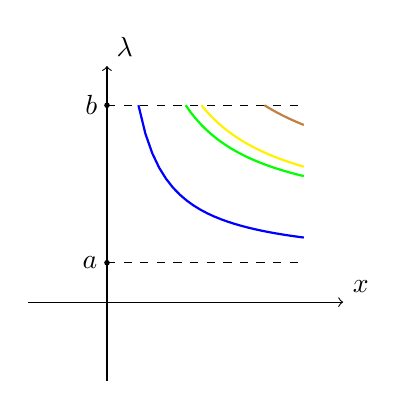
\begin{tikzpicture}
        \draw[->](-1, 0) -- (3, 0) node[above right] {$x$};
        \draw[->](0, -1) -- (0, 3) node[above right] { $\lambda$ };
        \draw[dashed] (0, 0.5) -- (2.5, 0.5);
        \draw[dashed] (0, 2.5) -- (2.5, 2.5);
        \fill (0, 0.5) circle(1pt) node[left] {$a$};
        \fill (0, 2.5) circle(1pt) node[left] {$b$};
        \draw[scale=1,domain=0.4:2.5,blue,thick] plot ({\x},{0.5 + 0.8/\x});
        \draw[scale=1,domain=1:2.5,green,thick] plot ({\x},{1 + 1.5/\x});
        \draw[scale=1,domain=1.2:2.5,yellow,thick] plot ({\x},{1 + 1.8/\x});
        \draw[scale=1,domain=2:2.5,thick,brown] plot ({\x},{1.25 + 2.5/\x});
    \end{tikzpicture}\]
    Непрерывная зависимость нулей от $\lambda$ следует из непрерывной зависимости решений от параметров и того, что все нули --- простые (кратности $1$).
\end{document}
